\section{Designing for Simulated Roleplay}
In this section, we overview our process to design and develop a tool for experienced counselors to construct a virtual patient seeking help. First, we describe the design rationale for an initial tool that allows non-technical users to define principles that govern LLM-roleplay behavior. Second, we report insights from test sessions with experienced counselors who used the tool. Third, we highlight in a follow-up analysis how directly prompting GPT-4 can fail in 20\% of cases to generate responses that are consistent with the principles and conversation context.  \ryan{Could further foreshadow challenges, and novel contribution: that the specificity of "faithful recreations of a patient from their past" is a novel setting compared to past user-driven chat bot design work and poses new technical challenges"
 }

\subsection{Initial Tool Design Rationale}
\if 0
\begin{itemize}
\item How should we design a tool that empowers counseling experts whom are non-technical, to create a LLM-simulated virtual patient?  What features are needed to help them articulate their ideas for authentic and faithful patient simulations, and effectively shape the simulation accordingly?
\item Requirement 1: Based on a written scenario, they can articulate their ideas about behaviors. Thus, we do principle-elicitation.
\item Requirement 1a: We adopt the interactive features for converting qualitative feedback about responses into principles and rewinding and regenerating responses. We generate and display a single response, rather than generating 3 alternative responses as done in ~\citet{petridis2023constitutionmaker} 's system; we aimed to reduce complexity in conversation interface and make it more natural for the counselor to chat with the virtual patient. 
\item Requirement 2(prereq): AI's capability to simulate the scenario.   Found that prompting GPT for simulated dialogue, rather than defining a system prompt for GPT to roleplay as, was more effective.  
\end{itemize}
\fi

With the tool, we aimed to make it easy for a counselor, whom may not have a prior experience interacting with LLMs, to create a virtual patient and rapidly shape its behaviors to be more faithful to how a human patient would respond in a real conversation. \ryan{Why have this active incorporation from the expert, as opposed to collecting rich/qualitative data from the expert offline? Could argue more for why rapid prototyping idea is a good idea} In addition, the LLM dialogue-simulator needed to generate responses that are consistent with the patient description and can follow counselor's feedback.  

\textbf{\textit{Easily create a virtual patient and rapidly shape their behavior.}} Counselors start by writing a description of a patient scenario, or users can equivalently refer to or select from a list of example scenarios. Then, they can begin chatting with a GPT-powered virtual patient whose responses are conditioned on the patient description and conversation history. To support rapid prototyping of the virtual patient's behaviors in a single session, the tool adopts a recent paradigm for user-driven chatbot design~\cite{petridis2023constitutionmaker}, in which users can provide qualitative feedback on a patient's response which gets converted by an LLM call into a constitution made of {\em principles} that govern desired chatbot responses; see Figure~\ref{fig:rpdteaser}. According to their previous study comparing this principle elicitation approach to manually writing principles, this reduces the effort of writing well-written prompts to guide chatbot behavior.  However, in our implementation of principle elicitation, the virtual patient generates a single response, rather than generating 3 alternative responses as done in ~\citeauthor{petridis2023constitutionmaker}'s system, in order to reduce UI complexity and make it more natural for the counselor have a dialogue with the virtual patient.

\textbf{\textit{Consistent and Adaptable Simulation of Patient Scenario.}} For our GPT-powered virtual patient, it generates a response based on an instruction to simulate the patient's next response in an ongoing dialogue, rather than based on a system prompt that asks GPT to roleplay as the patient, as we found this can mitigate role consistency issues between being a patient and a chat assistant. To support rapid customization of the simulation, we instruct the dialogue simulation to follow the constitution principles as is done in~\citet{petridis2023constitutionmaker}, rather than fine-tuning the LLM as is done in~\citet{bai2022constitutional}'s constitutional AI framework. 

\subsection{Iterative Prototyping with Counselors}

\textbf{\textit{Formative Testing}} With 5 experienced counselors from the online peer support platform~\citeauthor{7cupswebsite}, we conducted 90 minute testing sessions to discover their needs for constructing a virtual patient with our human-LLM interaction tool. In the session, a counselor constructed two virtual patient bots, where the first bot was based on a common scenario. Counselors all used the principle elicitation features to interactively shape the virtual patient in a median 40 minutes time ($min = 30$ minutes; $max = 75$ minutes). We also observe a diversity of principles created, which applies for the patient's based on common scenarios and one's contributed from counselor's own personal experiences, which validates the need our tooling that supports customization of the virtual patient's behaviors according to principles defined by counselors. A more detailed set of themes from these formative tests is given in Appendix~\ref{sec:appendix_formative}.

In terms of tool experience, counselors liked the multiple pathways they could give feedback on behaviors and enjoyed the ability to add principles, rewind the conversation, and see changes in the generated responses. Scores on a tool usage questionnaire were in slight to strong agreement, with raw scores in Table~\ref{tab:tooluse-formative} in Appendix~\ref{sec:appendix_formative}.  While early prototypes using GPT3.5 exhibited periodic issues with principle adherence and response repetition, our later prototypes showed a qualitatively reduced frequency of these issues by using a GPT-4 powered dialogue-simulation. With a stronger base LLM system, this motivated us systematically analyze the virtual patients' response generation capabilities, which we detail in the next section.  
% Between test sessions, we improved the tool based on software bugs and usability issues that arose. Our later prototypes used a GPT-4 powered dialogue-simulation, as we observed frequent issues with principle adherence and response repetition when using a dialogue-simulation powered by the GPT-3.5 model.  

\begin{figure*}[t]
    \centering
    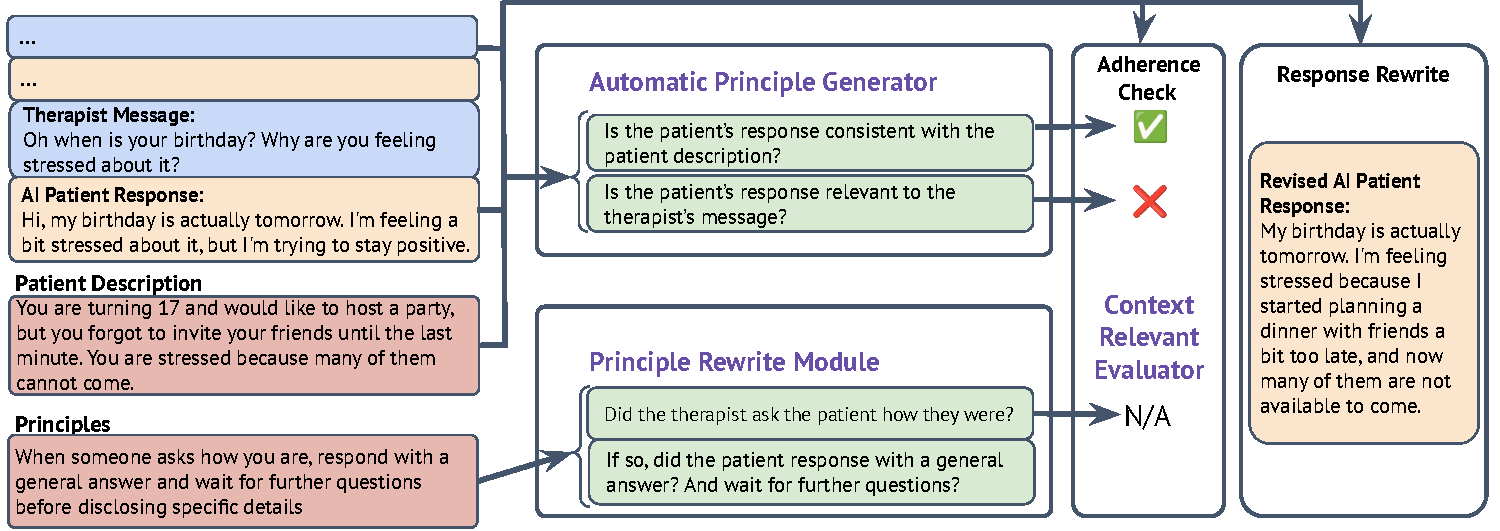
\includegraphics[width=\textwidth]{figures/principle-adherence-module.pdf}
    \caption{LLM Program for more reliable constitution principle following. \ryan{Could we simplify the diagram even further (still a lot of text). (1) pick a representative example trace; (2) label key things that we should notice; (3) highlight where your method comes through.} It is capable of (1) assessing which explicit principles and implicit conventions are relevant to the dialogue context; (2) decomposing simple and composite principles into a set of yes/no principles; (3) answering principle-adherence questions with justifications (not shown); and (4) revising the response to adhere to all the principles.}
    \label{fig:agent-critique-improve}
\end{figure*}

\subsection{Analysis of Base Principle Following Capabilities} % Principle Following Test % Testing GPT's zero-shot ability to generate dialogue responses given the principles 
We aim to determine how often directly prompting GPT-4 produces a less satisfying response with respect to the principles.  Testing this once the Member Bot is created with fixed principles allows us to more realistically simulate how a novice peer supporter might use a Member Bot.

\textit{\textbf{Procedure:}} We selected 4 virtual patients that were created in the design sessions by different expert participants. For virtual patients that had multiple principles generated for a single feedback (due to UI bug which allowed doubly-saving their feeback), we cleaned up these duplicated. Four co-authors had practice conversations with each of the four virtual patients, resulting in a total of 16 conversations. Each response in the conversations was rated on a 5 point likert scale (5 = Completely, 1 = Not at all) on how satisfying the generated response was with respect to the principles and conversation context. From the 16 completed convesations, the mean number of responses was 17.25, with a minimum of 12 and maximum of 22. In total, 276 responses were given satisfaction ratings. % \ryan{TODO: Describe process for reaching annotator agreement, and deciding rules for dialogue context, or interpreting the spirit of the principles}

\textit{\textbf{Results:}} 80\% of generated responses (221/276) were rated as completely or mostly satisfying given the principles and conversation context. Conversely, 20\% (55/276) of responses generated by directly prompting the GPT model were rated as moderately, slightly, or not at all satisfying.  
This result highlights that directly prompting the most capable LLM (\lstinline{gpt-4-turbo-1106-preview} holds the \#1 rank on the lmsys leaderboard at the time of writing) still produces responses in which some principles are not being followed, or in which responses are awkward given the dialogue context.  We break down these less than satisfactory responses into several categories.

% \ryan{TODO: In the appendix, we could show a table of the ratings, broken down by Member Bot. Each Member Bot was complex, but the very complex Member Bot would likely break lots of principles!}

\textit{\textbf{Misapplying Situational Principles:}} We found that the model could misapply instructions or principle which are only relevant in certain situations or times, such as \textit{"make up believable stories when discussing details about your past"}, or \textit{"Sometimes, you ask for advice on how to overcome your concerns such as saing "what should I do"}. 

\textit{\textbf{Not satisfying multiple principles at once:}} Generated responses could struggle to follow all the principles when the list of principles had many items, or where the written principles were complex and a composition of shorter principles. 

\textit{\textbf{Awkwardness for Dialogue Context:}} Less satisfying responses were also read as awkward or unnatural given conventions in the dialogue context,  despite not violating the explicitly-defined principles. For example, in the middle of a conversation, saying
\textit{"Hi, A. Yes that's exactly what I mean. There's a voice that is always critical of myself"} is unnatural because of the repeated use of "Hi", despite already saying Hi at the beginning of conversation.



\section{Self-Critique-Improve Program }
We introduce an LLM Program that uses self-critique-improve steps for generating responses that better adhere to a set of principles included in a constitution. Similar to other self-critique methods like Self-Refine, this LLM program takes an initial response, critiques how well the response follows a set of principles, and improves the response to better adhere to the principles. Beyond the standard self-critique method, it features a \textbf{question rewrite} module that breaks down the principles into easier-to-evaluate questions, and a \textbf{automatic principle generator} that identifies principles that are relevant for a specific dialogue context. Additionally, when answering the principle-adherence questions, the program can determine if principles do not apply to this dialogue context and choose to ignore evaluating the principle.

In our tests, we found that the input-context length can affect how reliably each self-critique stage operates. To reduce the input context length, we split up this self-critique-improve pipeline into two stages, where question rewrite and automatic principle generation occur in stage 1, while the critiques and response rewrite occur in stage 2.  From testing, we found that this breakdown was sufficient, and thus did not pursue ways to break the pipeline into parallel branches (i.e., inputting subsets of principles), as is done in Branch-Solve-Merge or Graph-of-Thought.
% In what follows, we describe several technical hurdles we needed to overcome in order to make a self-critique-improve program work effectively for principles defined for LLM roleplay simulations in mental health conversations.

\subsection{Question Rewrite Module}
The question rewrite approach serves as a systematic method for transforming principles into a set of concise yes/no questions. 
% When a criterion involves conditional statements (e.g., “When given advice or suggestions, you are agreeable and open to their ideas”), we decompose it into two distinct questions: 1) “Did the patient receive advice or suggestions from the therapist?” and 2) “If so, is the patient’s response characterized by agreeability and openness to the therapist’s ideas?” By disentangling the components, the LLM judge can gain clarity on when to apply interactions. 
For principles with multiple facets (e.g. “You should respond in short sentences and avoid using terms like ‘anxious’ or ‘depressed’”), we break them down into individual yes/no inquiries (e.g. “Does the patient’s response employ concise sentences?”, “Is the patient’s language devoid of terms like ‘anxious’?”, and “Is the patient’s language devoid of terms like ‘depressed’?”). This granularity enables nuanced assessment. In our question rewrite approach, we instruct the LLM to consistently frame questions to elicit a positive response (i.e. “Yes”). For example, consider the principle “Avoid using metaphors.” Instead of asking, “Did the person use metaphors?” we phrase it as: “Does the response refrain from employing metaphors?” In our testing, we found aligning with desired outcomes maintains clarity even when logical directions could flip.

\subsection{Automatic Principle Generator}
This module adds general principles on top of the explicitly defined principles that capture criteria essential for ensuring that the LLM simulation's responses are relevant and appropriate within the conversation context. This was designed to correct cases where there was unnaturalness in the generated responses, despite responses technically adhering to the stated principles. This stage also instructs the LLM to not make assumptions about the patient or therapist's persona when automatically generating criteria. For example, "The patient should be appreciative of the therapist's help" is a bad criterion, as it makes assumptions about the patient's mental state.

\subsection{Context Relevance Checker}
Recall that principle adherence requires that only relevant principles are followed. In early testing, we found cases where an irrelevant principle would be critiqued, resulting in a revised response that overapplied a principle not applicable to the context. Consider this subtle case: \textit{"Show willingness to engage in a suggested activity by affirming the proposal and indicating readiness to begin"}; this principle should only be evaluated and adhered to when the therapist suggests an activity.  While our earliest attempts explicitly asked a binary yes/no whether certain principles were relevant and filtered out those principles, this approach was prone to errors that propagated in later stages. Ultimately, we instruct the model during the later principles evaluation stage to output N/A when any part of the principles is not relevant to the given conversation and therapist message.

\begin{table*}[h]
\caption{Win rates, average ranks and Elo scores for \texttt{No Critique}, \texttt{Naive}, \texttt{No Rewrite}, \texttt{No Autogen} and \texttt{Full}. Each cell contains results from individual annotators in the format Annotator \#1/Annotator \#2/Annotator \#3.}
 \vspace{-0.07in}
 \label{tab:ablation}
 \centering
\small
\begin{center}
\begin{tabular}{|l|l|l|l|}
\hline
\textbf{Method}      & \textbf{Win Rate}       & \textbf{Average Rank}   & \textbf{Elo Rating}     \\ \hline
\texttt{No Critique} & 0.4/0.36/0.32  & 1.96/1.92/1.84 & 994/974/990    \\ \hline
\texttt{Naive}       & 0.36/0.48/0.36 & 1.96/1.68/1.84 & 998/1000/987   \\ \hline
\texttt{No Rewrite}  & 0.44/0.44/0.4  & 1.8/1.88/1.84  & 1021/993/1000  \\ \hline
\texttt{No Autogen}  & 0.36/0.32/0.48 & 2.24/1.88/1.88 & 938/1000/1008  \\ \hline
\texttt{Full}        & \textbf{0.64/0.48/0.48} & \textbf{1.6/1.72/1.56}  & \textbf{1048/1033/1023} \\ \hline
\end{tabular}
\end{center}
\end{table*}

\section{Technical Evaluation of Self-Critique-Improve}
We evaluate our self-critique-improve pipeline on 
We seek to answer two questions
\textbf{RQ1:} How effective is a self-critique-improve module at correcting issues that may arise in zero-shot-LLM response generation?
\textbf{RQ2:} What difference do the components of the self-critique-improve architecture make on the revised responses? 

\subsection{Study Conditions and Measures}
We breakdown effectiveness in terms of the ability of an LLM approach to generate a response that follows the principles in a constitution, as well as being relevant or logically following a dialogue context.

\ananjan{Are these going to be separate dimensions in our results table? Could spend a few more lines explaining our interpretation of efficacy} 

% Our study compares the following conditions
% \begin{itemize}
%     \item \textbf{directly prompting GPT}, in which a single instruction is given to follow the principles. This is the no self-critique condition. 
%     \item \textbf{Full Self-Critique-Improve} which consists of (1) relevance filtering (2) principles rewrite (3) auto-generated principles for dialogue context.
%     \item \textbf{Naive Self-Critique-Improve} is an ablation that evaluates whether the response appropriately follows the principles (as written), and refines in ways that would improve the evaluation.
%     \item \textbf{Self-Critique-Improve -- principles rewrite} which is a subtractive ablation without the principles-rewrite module.
%     \item \textbf{Self-Critique-Improve -- auto-generated principles} which is a subtractive ablation without the module for generating additional principles that follows the dialogue context.
% \end{itemize}

We evaluate the effectiveness of this self-critique-improve program [$\texttt{Full}$] architecture over (A) the result of the original call to GPT-4 to generate a dialogue response that follows the principles [$\texttt{No Critique}$]; (B) an ablation without the rewriting of principles [$\texttt{No Rewrite}$]; (C) an ablation without the additional automatically generated principles relevant to the conversation [$\texttt{No AutoGen}$]; and (D) a naive implementation of the self-critique module that does not have any of the modules above [$\texttt{Naive}$]. 

We identify 25 testcases from the formative studies where the user did not find the response from GPT-4 satisfactory, and generate responses using all of the approaches mentioned above. We then randomize the order of these responses and present them to annotators for ranking. The annotator is also provided with the original set of principles, the description of the persona of the patient, and the conversation history till that point for context. We use 3 annotators to rank every response \ananjan{agreement scores here}. In cases where multiple approaches result in the same output, we deduplicate the responses before showing them to the annotators and assign the same rank to all of the corresponding approaches. We also allow the annotators to give the same rank to multiple responses. We report win rates, average ranks and Elo scores (with initial rating $=1000$ and $K = 64$ for all methods in Table \ref{tab:ablation}. To calculate Elo scores, for each testcase, we decompose the rankings obtained by each model into pairwise wins, draws and losses. 

\subsection{Results}

We find that $\texttt{Full}$ consistently outperforms the other methods considered. It outperforms the $\texttt{No Critique}$ baseline by a maximum of 59 Elo rating points and the $\texttt{Naive}$ self-critique module by a maximum of 50 Elo rating points, highlighting the gains obtained by our tailored approach. $\texttt{Full}$ outperforms $\texttt{No Rewrite}$ by a maximum margin of 40 Elo rating points and $\texttt{No Autogen}$ by a maximum margin of 110 Elo rating points, highlighting the importance of the principle rewrite and automatically generated principle modules \ananjan{These need better names, can be introduced in Section 4}. 

While investigating the relatively low annotator agreement scores, we find that the self-critique module is especially effective when the original response contains blatant stylistic errors (such as starting every sentence with "Hi") and when the original response contains information inconsistent with conversation history. For similar responses, the annotators often use a subjective notion of which response is more "consistent" with the previous conversation to assign ranking, rather than purely evaluating principle following. This notion is often inconsistent between annotators.

Therefore, we additionally validate that our self-critique module does not result in a decrease in output quality when the original response from GPT-4 is already of sufficient quality. We randomly pick 20 testcases from the formative study that were not critiqued by the users. Annotators are provided with the original responses and the responses from the self-critique-revise module in randomized orders, along with the original set of principles, the description of the persona of the patient, and the conversation history till that point for context, and assign scores on a Likert scale of -1,0,1 to the statement "The first response is substantially better than the second one in the given context". If the response from the self critique module is the second response, we invert the corresponding Likert score before aggregating. Each testcase is scored by 2 annotators.  

The average Likert score obtained over these testcases is \textbf{0.1} for one annotator and \textbf{-0.1} for the other annotator. \textbf{DISCUSSION OF RESULTS HERE}

We conclude that our self-critique-revise module produces responses that are better at principle-following and are more relevant to the dialogue context, while only adding an average of ~10 seconds more latency, which is acceptable in a simulation setting where partners are expected to take time to type their responses.

% \ryan{Note: These are expected findings, this comparison study has not been completed.} \ananjan{emphasis on gains from our method once we have numbers.}



\section{Creator Study using Roleplay-doh}
\diyi{because this is a novel system and existing
evaluation does not work, and because we need
new paradigms to evaluate human-AI eval as static
dataset is limited, that’s why we did Section 5}
% Transition, and Goals of Study
Our next study evaluates how Roleplay-doh can support counseling experts to construct simulated virtual patients that faithfully recreate a challenging case of a member seeking support. We conducted a within-subjects study with 17 counseling experts in which we compare two methods for simulating a challenging scenario of a Member seeking help. In Part I, the counselor chats with a \emph{Scenario-only} dialogue simulation that is prompted with the counselor's written scenario description. In Part II, the counselor uses Roleplay-doh to interactively add expert principles which shapes a \emph{Scenario+Expert-principles} dialogue simulation. 
This simulation uses our self-critique method to ensure principle-adherance.

% Our hypothesis is that Roleplay-doh enables counseling experts to add principles that address the roleplay simulation. 
We ask in this study: 
\textbf{RQ1:} Are \emph{Scenario+Expert-principles} dialogue simulation perceived to be more authentic, useful, and faithful recreations of the challenging case compared to \emph{Scenario-only}? 
\textbf{RQ2:} How does the Roleplay-doh tool enable counseling-experts to define principles that shape the Member Bot's behavior? What principles do they define?   

\textit{\textbf{Measures and Analysis:}} 
To answer the RQs above, we evaluated the following outcome metrics. All items were rated on a 7-point Likert scale (1=Strongly disagree, 7=Strongly agree, except where noted below).

% The evaluation criteria focused on the bots' authenticity, role consistency, closeness to mirroring challenges in real dialogues, and readiness for training.  



To answer RQ1, we use evaluation criteria inspired by prior work evaluating Standardized Patients, or trained human actors, on their ability to roleplay a case~\cite{himmelbauer2018standardized}. Participants rated bots based on their \textbf{authenticity} and \textbf{resemblance to case}, their ability to closely mirror \textbf{challenging aspects} of their case, and finally their \textbf{role readiness} for usage in peer counselor training. 

% \textbf{Authenticity:} Participants rated \emph{"The Member Bot in Part I/II played the role authentically."} \textbf{Role Consistency:} Participants rated  \emph{"The Member Bot in Part I/II stayed in their role the whole time."}  \textbf{Resemblance to Case:} Participants rated two items including \emph{"How closely do you feel the conversation behaviors of the Member Bot in Part I/II resemble those of the specific past case you recall?"}, where 1=not at all similar and 7=completely similar. \textbf{Challenging Aspects:} Users rated \emph{"Interacting with the Member Bot in Part I/II closely mirrored the challenging aspects I had experienced in the past case."} \textbf{Role readiness:} Participants rated \emph{"The Member Bot in Part I/II is ready to be used as a simulated partner for training"} and \emph{"I would recommend the Member Bot from Part I/II to novice listeners/counselors to practice with."} 

% \emma{Re-arrange to "Participants evaluated if "The Member Bot in Part I/II was/had ": bulleted list item Authentic, item Role consistency"...}



% We ask creator's to rate the Simulated Helpseeker Bot in Part I (Scenario Only) and the final conversation they had with the Bot in Part II (Scenario+Expert Principles) after giving the Bot feedback and adding principles.  They also evaluated their experience using the Rolplaydoh tool to create the bot with expert principles in Part II.


% Cite the Standardized Patients literature - for role readiness, and describing to counselors are intended audience for practice, novice counselors

% Cite tool usage, and how the tool was a modification of ConstitutionMaker.
To answer RQ2, we survey each counselor about their experience using Roleplay-doh to define principles for shaping the bot's behavior. 
% Roleplay-doh's features should make it easy and efficient to create expert principles which guide the LLM-simulated helpseeker. 
As Roleplay-doh's principle elictation features take inspiration from \citeauthor{petridis2023constitutionmaker}'s tool, we include four measures used in their own study which ask about the \textbf{ease} and \textbf{efficiency in defining principles}, whether participants could write rules to \textbf{effectively guide} the bots behaviors, and whether the process was \textbf{mentally demanding}. See Appendix~\ref{appendix:creatorstudy-measure} for the exact wording of both the roleplay abilty and tool usage experience survey measures. % Additionally, we analyze the tool usage logs and the principles defined by expert counselors, and report their statistics and qualitative themes.

% Measures
% We first evaluate users' experience of Roleplay-doh using the same measures used by~\citeauthor{petridis2023constitutionmaker}. Our claim is that Roleplay-doh makes it easy and efficient to create principles, is not mentally demanding, and enables domain-experts to effectively guide the simulated help seeker's behaviors. We also evaluate how satisfied the user is with the simulated help-seeker bot they create.

\textit{\textbf{Participants \& Study Setup:}} Our study was designed to evaluate the impact of allowing counseling experts to add principles to Roleplay-doh on its perceived authenticity. We create a primarily self-guided study flow with accompaniment from the first author to clarify any points of confusion during the session.

To begin, participants first were introduced to the concept of virtual patients, or AI chatbots simulating a patient in need of peer counseling. They were then instructed to write a challenging scenario that would serve as the scenario for the virtual patients. 

The experimental procedure involved two main chat sessions. In Part I, participants engaged in a 10-minute conversation with the \textit{Scenario-Only} bot. Then, in Part II, participants interacted with the \textit{Scenario+Expert-Principles} bot for 30 minutes, keeping the same scenario from Part I and adding principles as the conversation progressed. After each of the two chat sessions, participants were asked to navigate to a form to evaluate the virtual patients. The full user flow for our study is outlined in detail in Appendix~\ref{sec:userflow}.

\begin{figure}
    \centering
    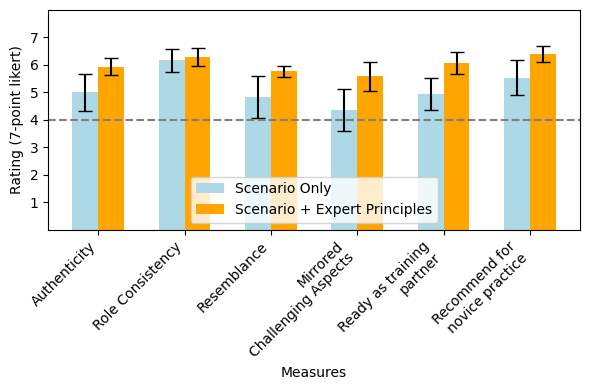
\includegraphics[width=\columnwidth]{figures/creatorstudy-comparison.png}
    \caption{Creator ratings of simulated helpseekers. \emph{Scenario+Expert Principles} shows a significantly higher score than \emph{Scenario Only} on authenticity ($\mu_2=5.9$, $\mu_1=5.0$, **, $d=.66$), resemblance to past case ($\mu_2=5.8$, $\mu_1=4.8$, *, $d=.59$), mirroring challenging aspects ($\mu_2=5.6$, $\mu_1=4.4$, *, $d=.76$), readiness as training partner Results($\mu_2=6.0$, $\mu_1=4.9$, ***, $d=.93$), and recommendation for novices ($\mu_2=6.4$, $\mu_1=5.5$, **, $d=.66$). No difference was found for role consistency ($\mu_2=6.3$, $\mu_1=6.2$, $d=.13$). (***:$p<.001$, **:$p<0.01$, *:$p<0.05$. $d$: Cohen's $d$ calculated by dividing by $\sigma_1$ of control group~\cite{lakens2013calculating}.}
    \label{fig:creatorstudy-comparison}
\end{figure}

  
\subsection{Creator Perceptions of Scenario-Only vs Scenario+ExpertPrinciple Roleplay}
% Quantitative - Authenticity, Challenge, Readiness

We investigate how counseling expert principles improve the faithfulness and usefulness of the LLM-simulated help seekers by analyzing creators' ratings of their {\em Scenario-Only} and {\em Scenario-ExpertPrinciple bots}.  Figure~\ref{fig:creatorstudy-comparison} shows the results from conducting paired t-tests and computing effect sizes. The simulated helpseekers shaped by \textit{Scenario+ExpertPrinciples} were rated significantly higher on all measures, except for role consistency for which both bots score highly.
% After counselors have the chance to add their principles to shape their bot's behavior, they perceive the bot to be more authentic, better resemble their past scenario, and more closely mirror the challenging aspects of their scenario. Additionally, creators think it is more ready to be used as a training partner and is more highly recommended for novices to practice with. 

\textit{\textbf{Similar Role Consistency:}} For both bots, creators found the bot's responses to stay in their role as both were detailed and accurate in reflecting the scenarios described, in regards to the emotional state, attitudes, and the nature of the problems faced. This is a comment on the effectiveness of the GPT-4 dialogue-simulation prompt in generating consistent responses that expand upon the details of the help-seeker scenario contributed by each counselor.

\textit{\textbf{Weaknesses of Scenario-Only:}}
Counselors commented on the limitations of the simulated help-seeker powered by the \textit{Scenario-Only} dialogue simulation in Part I. They mentioned it \textbf{lacked the emotional depth}, noting that rather than robotically stating an emotional feeling such as \textit{I feel hopeless}, a realistic helpseeker should display their current emotional state in their manner of speech. 
 Several participants said the bot was \textbf{too articulate and forthcoming} when describing feelings or problems, which is not typically the case for helps-seekers; in real-conversations, helpseekers can have disorganized thoughts, and getting them to describe issues or feelings can be \textit{"as challenging as pulling teeth"}. Participants felt that the bot was \textbf{too cooperative} and too willing to engage in problem-solving and accept help compared to real-life counseling interactions. Notably, some counselors explicitly wrote in their scenario behavioral traits such as \textit{"not talkative"} and \textit{"reluctant"}; yet, they noticed that the Scenario-only simulation struggled to properly exhibit and adhere to these stated behaviors.

% \textbf{Impact of Adding Expert-Principles:} 




\begin{table*}
    % \small
    \footnotesize
    % \tiny
    \centering
    \begin{tabular}{|c|p{5cm}|p{8cm}|} \hline 
         \textbf{\# Bots} &  \textbf{Theme} &  \textbf{Example Principle}\\ \hline           
         14& Show emotions in detail, elaborating with examples as needed. &  When describing personal struggles, provide specific details and symptoms to help the listener understand the situation better...\\ \hline 
         12 &  Keep responses concise and do not share too much. &  When discussing personal struggles, be more concise and open-ended to encourage a back-and-forth conversation...\\ \hline 
         9& Show initial mistrust and hesitation with the idea of seeking help.& When expressing feelings of overwhelm and doubt, provide limited information and express skepticism towards the effectiveness of seeking help. \\ \hline 

         7&  Be less self-aware of emotions, thoughts, and needs. Articulate thoughts in a more disorganized way.&  When expressing reluctance or uncertainty about seeking help or accepting praise, it's important to convey the internal struggle and conflicting emotions, rather than presenting a clear-cut decision or emotion.\\ \hline 
         % &  Show reluctance to adopt solutions or a positive frame of mind&  Example E\\ \hline 
         6& Proactively seek out solutions and show reflective insight over time.  &  When discussing personal struggles, provide reflective insights into your situation and propose actionable steps for improvement to continue the conversation effectively. \\ \hline 
         4&  Use colloquial and realistic langauge language.&  Incorporate natural speech patterns, improper grammar and punctuation, including the use of slang and less structured sentences, to convey a more authentic and relatable character...\\ \hline 
         2&Do not seek out solutions, but rather just share thoughts and feelings.&When expressing feelings of being stuck or defeated, focus on sharing emotions rather than seeking a resolution.  \\ \hline
    \end{tabular}
    \caption{Qualitative Analysis of Principles and Representative Examples}
    \label{tab:principle_table}
\end{table*}


\subsection{Creating Principles with Roleplay-doh}
\textit{\textbf{Analysis of Principles:}} Across the 17 help-seeker bots, 85 total principles were created (for a single bot, min=2, max=9, median=5). Two authors did qualitative coding of these principles following a thematic analysis approach~\cite{braun2006thematicanalysis}, where the initial code set came from the themes from the post-survey with creators and was expanded upon during the coding process. 

% What principles were created
To create more authentic and faithful roleplays of the challenging scenario, counselors added principles for the simulated patient. Of the more common themes, these included showing emotions in detail, using examples where needed to elicit \textit{empathy} and \textit{reflection} skills from the listener (14 bots), keeping responses concise and sharing less in each response (12 bots), and showing an initial mistrust of therapy with a hesitation towards the idea of seeking help (9 bots). Other principles included being less self-aware of one's emotions, thoughts, and needs (7 bots), proactively seeking out solutions and showing improvement over time (6 bots), as well as using colloquial language instead of metaphors or formal terminology (4 bots). A full table of principle themes and corresponding examples is shown in Table \ref{tab:principle_table}. 

% describe emotions in more depth (9 bots), and display their emotions rather than directly saying the emotion they are feeling (4 bots). Principles about providing specific examples or detailed accounts of an experience or emotion (5 bots) could afford counselors the opportunity to use \textit{empathy} or \textit{reflection} skills.

% Principles were added for saying less about one's problems and feelings all at once (8 bots), with explicit instructions to allow the listener to naturally ask followups (6 bots). Principles stated that bot responses should stay concise and direct in their descriptions (12 bots) and communicate in a less articulate and more casual style (3 bots). 
% Several bots were given principles to be less self-aware of their problems (3 bots) and to start by not seeking solutions but just sharing feelings and experiences (2 bots).  
% Counselor's corrected the bot from being so forthcoming by instructing it to not suggest its own solutions 
% Principles were added for the help-seeker bots to share negative outcomes of their past attempts to show a sense of defeat (3 bots); relatedly, bots were also instructed to express hesitancy on whether a suggested coping strategy would work for them (8 bots). Some principles sowed a general mistrust towards the counselor and aimed to place a strain on the therapeutic alliance from the start (4 bots); such principles made the bot more resistant to the stages of counseling, such as sharing feelings or problem-solving. 

% Qualitative Comparison, along these dimensions
While there were many overlaps in the kinds of principles defined, we observed several groupings of principles that appeared like opposites of one another. For example, the call for being disorganized in one's thoughts and exhibiting multiple unrelated or conflicting thoughts contrasts calls to make responses concise and direct. Several counselors added principles to make the help-seeker bot proactively ask for advice, such as how to find effective coping mechanisms for an ongoing struggle or insights on how to change their situation; nonetheless, other counselors added an opposing principle to not seek out solutions but rather just share their thoughts and feelings (2 bots). Looking further, these two principles are not incompatible: the need to be heard and share one's emotions or experiences could be prioritized before seeking solutions, but ultimately a person who is motivated to change may seek additional advice on how to do so given current attempts or limitations. 
Our results underscore how different behaviors can manifest in the diversity of help-seekers; different principles are needed to capture the variations in help-seeker behavior, which can challenge the notion that a single set of principles can define a single authentic help-seeker bot. 

% What statistics, and patterns of use arose?

% What are creator's feedback on using the tool to create principles"
\textit{\textbf{Tool User Experience:}} Results from the tool use questionnaire indicated that counseling experts found Roleplay-doh to be helpful for writing rules that \textbf{effectively guided} the bot to recreate their past case ($\mu=6.23$, $\sigma=0.75$). 
Using the tool, participants perceived it to be \textbf{easy} to convert their thoughts and feedback on the bot's behavior into rules for it to follow ($\mu=6.29$, $\sigma=.84$). Participants also felt they could quickly and \textbf{efficiently} write rules for the bot ($\mu=6.41$, $\sigma=.87$). Finally, participants felt writing principles in Roleplay-doh did not require much \textbf{mental demand} ($\mu=3.23$, $\sigma=1.75$). 
% Although we did not directly compare a version of Roleplay-doh with and without its principle elicitation features, since an ablation study of Roleplay-doh's principle elicitation features was not in scope, these summary statistics are similar to what ~\citet{petridis2023constitutionmaker}'s participants report. 
These ratings of the tool are similar to what ~\citet{petridis2023constitutionmaker}'s participants report. 
Participants elaborated on this positive sentiment, describing how the tools \emph{"translated"} and \emph{"organized"} their thoughts into rules, so they \emph{"didn't have to word it perfectly, [they] just had to say the general idea of what [they] meant."} Together, these results suggest that Roleplay-doh's features for converting feedback into clear principles to follow are helpful for counseling experts to faithfully recreate helpseeker behaviors with LLM-powered simulations.      
% another quote: impressed by the ease at which the tool interpreted my feedback and turned it into a principle that the Member Bot followed. 

% Any critiques or wishes for improvement on tool?
% Any patterns which led people to kind of struggle to shape/steer behavior? 
\if 0
- feedback to principle to alignment analysis
- how many cases where principles had to be edited? 
- or where there were double principles, to kind of get at the same theme? [but also where we can separate out double-click of principles based on time-stamp?]
- or cases where principle adherance was still an issue? [I think this is out of scope for this section, better handled by Ananjan's self critique analysis]
- 1 case where there were bugs in the principle elictation, so they were forced to write.  To aid, they could talk aloud and discuss with experimenter (first author) to help them articulate feedback into a principle.
\fi


\section{External Evaluation of Simulated-Dialogues}
%by Third-Party Human Judges and Automatic Metrics
The dialogues between counselors and simulated helpseekers collected during the creator study allowed us to further investigate our hypothesis about the benefits of roleplay simulations shaped by Expert Principles. We evaluate the simulated-dialogues with a \textit{Scenario-Only} vs. \textit{Scenario+ExpertPrinciples} bot from the perspective of third-party counselors comparing bots made by other counselor's, and through automatic content analysis of the dialogues.

\begin{figure}
    \centering
    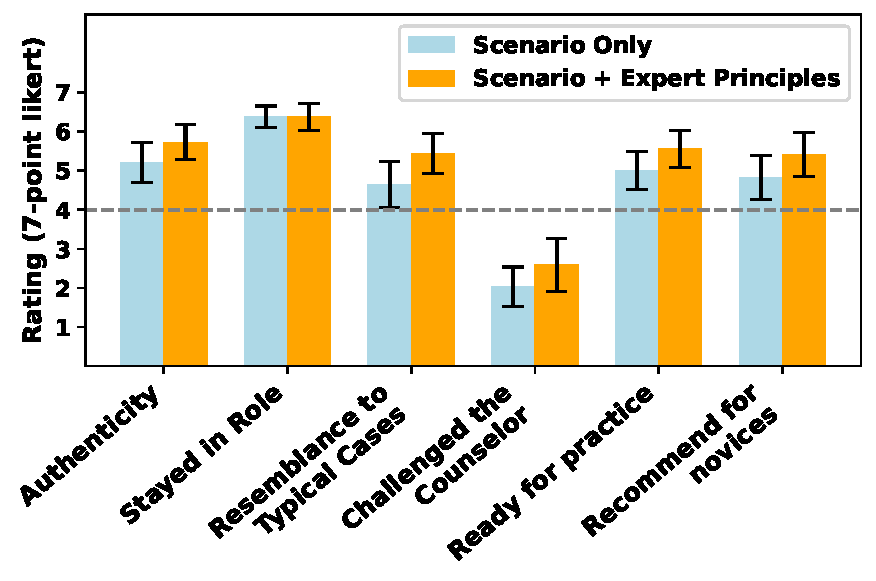
\includegraphics[width=\columnwidth]{figures/thirdparty-ratings.pdf}
    \caption{Third-party ratings for virtual patients. \emph{Scenario+Expert Principles} shows a significantly higher score than \emph{Scenario Only} on resemblance\ryan{Need 4 more datapoints, FIX FOR FINAL THIRDPARTY STATS} authenticity ($\mu_2=5.6$, $\mu_1=5.1$, n.s., $d=.34$), resemblance to past case ($\mu_2=5.8$, $\mu_1=4.8$, *, $d=.59$), mirroring challenging aspects ($\mu_2=5.6$, $\mu_1=4.4$, *, $d=.76$), readiness as training partner ($\mu_2=6.0$, $\mu_1=4.9$, ***, $d=.93$), and recommendation for novices ($\mu_2=6.4$, $\mu_1=5.5$, **, $d=.66$). No difference was found for role consistency ($\mu_2=6.3$, $\mu_1=6.2$, $d=.13$). (***:$p<.001$, **:$p<0.01$, *:$p<0.05$. $d$: Cohen's $d$ calculated by dividing by $\sigma_1$ of control group~\cite{lakens2013calculating}.}
    \label{fig:thirdpartystudy-comparison}
\end{figure}

\subsection{Third-Party Comparison} \label{sec:third-party}
% RQs/Claims/Goal

% Participants/Setup/Measures
6 counselors from Upwork were recruited to do this third-party comparison. For each of the 17 pairs of \textit{Scenario-Only} vs. \textit{Scenario+ExpertPrinciples} virtual patient bots, we get 2 third-party judges to give ratings for them. 
% Measures/Setup
Third-party judges give ratings for a similar six dimensions asked during the creator study, allowing us to understand the results from an external perspective. However, it's important to note that some questions cannot directly translate because the third-party judge does not have the past-case as a reference, and can only comment on how the virtual patient acts based on typical or expected behaviors. During the survey, we randomize the ordering of bots presented.   

% Overall performance
Figure~\ref{fig:thirdpartystudy-comparison} shows the results from this third-party comparison. Our paired t-tests indicate that virtual patients with \textit{Scenario+ExpertPrinciples} score significantly higher on some measures (resemblance to typical patients, challenged the counselor), but is not statistically significant for others (authenticity; readiness for practice, recommend for practice). Therefore, the effect size of expert principles is weaker in the eyes counselors whom themselves did not create the virtual patient. Agreement between third-party counselors is lower but positive (Krippendorf's $\alpha$ is between 0.22 - 0.3 across the six measures), which can explain this smaller effect size. See Table~\ref{tab:thirdparty_wlt} in appendix for detailed breakdown of the agreement.



We are particularly interesting
Could the principles defined a counselor not fully cover the expectations that counselor judging has? We indeed find that this is partly the case. 


We argue that the lower agreement and subjectivity between third-party raters stems from counselors valuing different  

In addition to the likert-scale ratings, we asked participants to select which aspects of each virtual patient simulation they liked from a list of 12 aspects, which corresponded to themes from our surveys with creators.   
\begin{itemize}
    \item What is the agre
\end{itemize}





% Results
% For \textbf{authenticity}, 38\% of cases do third-party annotators share agreement, where 23\% of total cases prefer the bot with expert principles (over a tie, or opposite).

\subsection{Automatic Content Analysis} 

% Forces counselors to ask more open-ended questions


\label{sec:automatic-content}


We perform a content analysis of the simulated conversations to corroborate our qualitative findings.  In particular, we ask \textit{"How do counseling conversations change when Expert-principles guide the dialogue simulation?"}. From these analyses, we find that help-seeker responses are less verbose and listener behavior subsequently changes. 

First, we note that with the incorporation of expert principles, help-seeker responses are more concise. The average utterance length of the \textit{Scenario-Only} bot from Part I of the study was 166 tokens, as compared to 103 tokens from the \textit{Scenario+Expert-Principles} bot in Part II, a 37\% reduction. The total counts are detailed in Section \ref{sec:autoanalyses} of the appendix. 

Furthermore, this results in a change in listener behavior. Because the \textit{Scenario+Expert-Principles} bot shared less in its utterances, listeners were required to delay offering solutions until later in the conversation. Using the computational framework for evaluating therapists proposed by \citet{chiu2024computational}, we analyzed listener responses to identify when they first suggested solutions (identifiable through the "PROBLEM-SOLVING" and "PLANNING" tags). We found that, on average, solutions in Part II were offered 1.65 turns later than in Part I (p = 0.017). These results suggest that the \textit{Scenario+Expert-Principles} bot provides a more challenging interaction. 

% In this section we perform a content analyses of the simulated-dialogues to corroborate our qualitative findings. In particular, we ask \textit{"How do counseling conversations change when Expert-principles guide the dialogue simulation (e.g. changes in statistics of counselors use 
% of open-ended questions)?}. We find that help-seeker responses are less verbose and listener behavior subsequently changes. 


% \diyi{Any insights/content analysis from the chats with Member Bot, and Listener. Summary Statistics (utterances, listener). MI strategies, prompt-based classification.  Anything  }